\documentclass[11pt]{scrreprt}
\usepackage[utf8]{inputenc}
\usepackage{graphicx}
\usepackage{listings} %插入代码
\usepackage{xcolor} %代码高亮
%\usepackage[demo]{graphicx}
\usepackage{caption}
\usepackage{tabularx}
\usepackage[labelformat=simple]{subcaption}
\usepackage{amsmath}

\renewcommand\thesubfigure{(\alph{subfigure})} % see subcaption doc

\lstset{numbers=left, %设置行号位置
	numberstyle=\tiny, %设置行号大小
	keywordstyle=\color{blue}, %设置关键字颜色
	commentstyle=\color[cmyk]{1,0,1,0}, %设置注释颜色
	frame=single, %设置边框格式
	escapeinside=``, %逃逸字符(1左面的键),用于显示中文
	breaklines, %自动折行
	extendedchars=false, %解决代码跨页时,章节标题,页眉等汉字不显示的问题
	xleftmargin=2em,xrightmargin=2em, aboveskip=1em, %设置边距
	tabsize=4, %设置tab空格数
	showspaces=false %不显示空格
}

\title{\textbf{Project 3 Report}}
\subtitle{CS325 Analysis of Algorithms, Summer 2015}
\author{\textsf{\textbf{Project Group 1}}\\
		\textsf{Tingzhi Li}\\
		\textsf{Nicholas Nelson}\\
		\textsf{Chunyang Zhang}}
\date{}

\begin{document}
\maketitle

\chapter{Transshipment Model}
\section{Part A}
The transshipment model is an extension of the transportation model. 
In addition to the standard transportation model, there are now 
intermediate transshipment points added between the sources (plants) 
and destinations (retailers). Items being shipped from a Plant 
($p_i$) must be shipped to a Warehouse ($w_j$) before being shipped 
to the Retailer ($r_k$). Each Plant will have an associated supply 
($s_i$) and each Retailer will have a demand ($d_k$). The number of 
plants is $n$, number of warehouses is $q$ and the number of 
retailers is $m$. The edges $(i,j)$ from plant ($p_i$) to warehouse 
($w_j$) have associated costs denoted $cp(j,k)$.

\subsection{i. Linear Formulation}

The objective function and constraints for this problem are as 
follows:

\begin{itemize}
	\item Minimize
[$10x_{1,1}+15x_{1,2}+11x_{2,1}+8x_{2,2}+13x_{3,1}+8x_{3,2}+9x_{3,3}+14x_{4,2}+8x_{4,3}+5y_{1,1}+6y_{1,2}+7y_{1,3}+10y_{1,4}+12y_{2,3}+8y_{2,4}+10y_{2,5}+14y_{2,6}+12y_{3,5}+12y_{3,6}+6y_{3,7}$] 
where $x_{i,j}$ represents number of refrigerators to be shipped 
from plant $i$ to warehouse $j$, and $y_{j,k}$ represents number of 
refrigerators to be shipped  from warehouse $j$ to retailer $k$.
	\item Supply constraints:
	\begin{enumerate}
		\item $x_{1,1} + x_{1,2} <= 150$
		\item $x_{2,1} + x_{2,2} <= 450$
		\item $x_{3,1} + x_{3,2} + x_{3,3} <= 250$
		\item $x_{4,2} + x_{4,3} <= 150$
	\end{enumerate}
	\item Retailer constraints:
	\begin{enumerate}
		\item $y_{1,1} >= 100$
		\item $y_{1,2} >= 150$
		\item $y_{1,3} + y_{2,3} >= 100$
		\item $y_{1,4} + y_{2,4} + y_{3,4} >= 200$
		\item $y_{2,5} + y_{3,5} >= 200$
		\item $y_{2,6} + y_{3,6} >= 150$
		\item $y_{3,7} >= 100$
	\end{enumerate}
	\item The number of refrigerators shipped into any individual 
		warehouse has to be equal to the number of refrigerators 
		shipped out from that warehouse, thus constrained by:
	\begin{enumerate}
		\item $x_{1,1} + x_{2,1} + x_{3,1} - y_{1,1} - y_{1,2} - y_{1,3} - y_{1,4} = 0$
		\item $x_{1,2} + x_{2,2} + x_{3,2} + x_{4,2} - y_{2,3} - y_{2,4} - y_{2,5} - y_{2,6} = 0$
		\item $x_{3,3} + x_{4,3} - y_{3,4} - y_{3,5} - y_{3,6} - y_{3,7} = 0$
	\end{enumerate}
\end{itemize}

\subsection{ii. Optimal Solution and Linear Program}

The optimal solution for this problem is as follows:\\

Objective value: 17100\\

\begin{tabular}{|c|c|c|c|c|c|c|c|c|c|}
	\hline variables & $x_{1,1}$   &  $x_{1,2}$ & $x_{2,1}$ & $x_{2,2}$ & $x_{3,1}$ & $x_{3,2}$ & $x_{3,3}$ & $x_{4,2}$ & $x_{4,3}$      \\
	\hline optimal value & 150  &  0 & 200 & 250 & 0 & 150 & 100 & 0 & 150            \\
	\hline
\end{tabular} \\

\begin{tabular}{|c|c|c|c|c|c|c|c|c|c|c|c|c|}
	\hline variables & $y_{1,1}$ & $y_{1,2}$ & $y_{1,3}$ & $y_{1,4}$ & $y_{2,3}$ & $y_{2,4}$ & $y_{2,5}$ & $y_{2,6}$ & $y_{3,4}$ & $y_{3,5}$ & $y_{3,6}$ & $y_{3,7}$  \\
	\hline optimal value & 	100 & 150 & 100 & 0 & 0 & 200 & 200 & 0 & 0 & 0 & 150 & 100 \\
	 \hline
\end{tabular} \\

Lindo Code
\begin{lstlisting}[language=c]
min 10x11+15x12+11x21+8x22+13x31+8x32+9x33+14x42+8x43+5y11+6y12+7y13+10y14+12y23+8y24+10y25+14y26+14y34+12y35+12y36+6y37
ST
	x11 + x12 <= 150
	x21 + x22 <= 450
	x31 + x32 + x33 <= 250
	x42 + x43 <= 150

	y11 >= 100
	y12 >= 150
	y13 + y23 >= 100
	y14 + y24 + y34 >= 200
	y25 + y35 >= 200
	y26 + y36 >= 150
	y37 >= 100

	x11 + x21 + x31 - y11 - y12 - y13 - y14 = 0
	x12 + x22 + x32 + x42 - y23 - y24 - y25 - y26 = 0
	x33 + x43 - y34 - y35 - y36 - y37 = 0
\end{lstlisting}

\subsection{iii. Optimal Shipping Routes/Minimum Costs}
The optimal shipping routes, based upon minimizing costs, are as follows: \\

\begin{tabular}{|c|c|}
	\hline From plants to warehouses & From warehouses to retailers \\
	\hline $x_{1,1} = 150$ & $y_{1,1} = 100$ \\
	\hline $x_{2,1} = 200$ &$y_{1,2} = 150$ \\
	\hline $x_{2,2} = 250$ &$y_{1,3} = 100$ \\
	\hline $x_{3,2} = 150$ &$y_{2,4} = 200$ \\
	\hline $x_{3,3} = 100$ & $y_{2,5} = 200$  \\
	\hline $x_{4,3} = 150$ & $y_{3,6} = 150$  \\
	\hline & $y_{3,7} = 100$ \\
	\hline
\end{tabular} \\

Minimum cost = \$17,100

\section{Part B}
Due to old infrastructure, warehouse 2 is going to close eliminating 
all of the associated routes. Therefore, all calculations as to the
optimal shipping route and minimized costs must be re-evaluated. The 
feasability of shipping all refrigerators to either warehouse 1 or 3
and then to the retailers without using warehouse 2 must also be
evaluated.

\subsection{Evaluation}
Without warehouse 2, there is no optimal solution to the transshipment 
model. It is not feasible to ship all refrigerators to either warehouse
1 or 3 and then to the retailers without using warehouse 2. Even if 
plants $p_3$ and $p_4$ shipped all refrigerators to warehouse $w_3$, 
the demands from $r_5$, $r_6$ and $r_7$ would not be met because
$p_3 + p_4 < r_5 + r_6 + r_7$.

\section{Part C}
Instead of closing warehouse 2, management has decided to keep a 
portion of it open but limit shipments to 100 refrigerators per week. 
The feasability of this model must be evaluated, and an optimal 
solution determined.

\subsection{Evaluation}
With warehouse 2 limited to 100 refrigerators per week, the model is
feasible. The optimal shipping routes, based upon minimizing costs, 
are as follows: \\

\begin{tabular}{|c|c|}
	\hline From plants to warehouses & From warehouses to retailers \\
	\hline $x_{1,1} = 150$ & $y_{1,1} = 100$ \\
	\hline $x_{2,1} = 350$ & $y_{1,2} = 150$ \\
	\hline $x_{2,2} = 100$ & $y_{1,3} = 100$  \\
	\hline $x_{3,3} = 250$ & $y_{1,4} = 150$  \\
	\hline $x_{4,3} = 150$ & $y_{2,4} = 50$  \\
	\hline 				  & $y_{2,5} = 50$ \\
	\hline 				  & $y_{3,5} = 150$ \\
	\hline 				  & $y_{3,6} = 150$ \\
	\hline 				  & $y_{3,7} = 100$ \\
	\hline
\end{tabular} \\

Minimum cost = \$18300

\section{Part D}
The generalized linear programming model for the transshipment problem 
can be expressed using the following formulation, objective function,
and constraints:\\

Objective function:
\begin{displaymath}
\min \left(\sum_{i=1}^{n} \sum_{j=1}^{q} cp(i,j)x_{ij} + \sum_{j=1}^{q} \sum_{k=1}^{m} cw(j,k)y_{jk}\right)
\end{displaymath}

$x_{ij}=0 \textrm{ if } cp(i,j) \textrm{ is not applicable, }$

$y_{jk}=0 \textrm{ if } cw(j,k) \textrm{ is not applicable,}$

where $x_{ij}$ represents the number of refrigerators to be shipped 
from plant $i$ to warehouse $j$ and $y_{jk}$ represents number of 
refrigerators to be shipped from warehouse $j$ to retailer $k$.\\

The constraints for this problem are as follows:

\begin{itemize}
	\item Supply constraints:
	\begin{displaymath}
	\sum_{j=1}^{q} x_{ij} \leq s_i 
	\qquad\textrm{where } i=1,2,\cdots,n
	\end{displaymath}
	\item Retailer constraints:
	\begin{displaymath}
	\sum_{j=1}^{q} y_{jk} \leq d_k 
	\qquad\textrm{where } k=1,2,\cdots,m
	\end{displaymath}
	\item The number of refrigerators shipped into any individual 
	warehouse has to be equal to the number of refrigerators 
	shipped out from that warehouse, thus constrained by:
	\begin{displaymath}
	\sum_{i=1}^{n} x_{ij} = \sum_{k=1}^{m} y_{jk} 
	\qquad\textrm{where } j=1,2,\cdots,q
	\end{displaymath}
\end{itemize}




\chapter{A Mixture Problem}

\section{Part A}
Veronica the owner of Very Veggie Vegeria is creating a new 
healthy salad that is low in calories but meets certain 
nutritional requirements. A salad is any combination of the 
following ingredients:\\

Tomato, Lettuce, Spinach, Carrot, Smoked Tofu, Sunflower Seeds, Chickpeas,
Oil\\

Each salad must contain:

\begin{itemize}
	\item At least 15 grams of protein
	\item At least 2 and at most 8 grams of fat
	\item At least 4 grams of carbohydrates
	\item At most 200 milligrams of sodium
	\item At least 40\% leafy greens by mass
\end{itemize}

The nutritional contents of these ingredients (per 100 grams)
and cost are:

\begin{figure}[!htbp]
	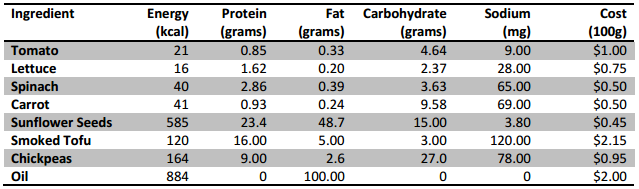
\includegraphics[width=1.0\textwidth]{nutritional.png}
\end{figure}

\subsection{i. Linear Formulation}
The objective function and constraints for this problem are as 
follows:

\begin{itemize}
	\item Minimize
[$21x_{1}+16x_{2}+40x_{3}+41x_{4}+120x_{5}+585x_{6}+164x_{7}+884x_{8}$]
where $x_{i}$ represents the weight (in kgram units) for ingredient $i$.
	\item Constraints
	\begin{enumerate}
		\item At least 15 grams of protein:\\
		$0.85x_{1}+1.62x_{2}+2.86x_{3}+0.93x_{4}+23.4x_{5}+16.00x_{6}+9.00x_{7} >= 15$
		\item At least 2 grams of fat:\\
		$0.33x_{1}+0.20x_{2}+0.39x_{3}+0.24x_{4}+48.7x_{5}+5.00x_{6}+2.6x_{7}+100.00x_{8} >= 2$
		\item At most 8 grams of fat:\\
		$0.33x_{1}+0.20x_{2}+0.39x_{3}+0.24x_{4}+48.7x_{5}+5.00x_{6}+2.6x_{7}+100.00x_{8} <= 8$
		\item At least 4 grams of carbohydrates:\\
		$4.64x_{1}+2.37x_{2}+3.63x_{3}+9.58x_{4}+15.00x_{5}+3.00x_{6}+27.0x_{7} >= 4$
		\item At most 200 milligrams of sodium:\\
		$9.00x_{1}+28.00x_{2}+65.00x_{3}+69.00x_{4}+3.80x_{5}+120.00x_{6}+78.00x_{7} <= 200$
		\item At least 40\% leafy greens by mass:\\
		$x_{2}+x_{3}-0.4x_{1}-0.4x_{2}-0.4x_{3}-0.4x_{4}-0.4x_{5}-0.4x_{6}-0.4x_{7}-0.4x_{8} >= 0$
	\end{enumerate}
\end{itemize}

\subsection{ii. Optimal Solution and Linear Program}

The optimal solution for this problem is as follows:\\

Objective value: 114.7541\\

\begin{tabular}{|c|c|c|c|c|c|c|c|c|}
	\hline variables & $x_{1}$ & $x_{2}$ & $x_{3}$ & $x_{4}$ & $x_{5}$ & $x_{6}$ & $x_{7}$ & $x_{8}$ \\
	\hline optimal value & 0 & 58.54801 & 0 & 0 & 0 & 87.82201 & 0 & 0 \\
	\hline
\end{tabular} \\

{\it Note:} The units for the objective value are kcal and the variables are in grams.\\

Lindo Code
\begin{lstlisting}[basicstyle=\small,language=c]
min 21x1+16x2+40x3+41x4+585x5+120x6+164x7+884x8
ST
	0.85x1 + 1.62x2 + 2.86x3 + 0.93x4 + 23.4x5 + 16.00x6 + 9.00x7 >= 15
	
	0.33x1 + 0.20x2 + 0.39x3 + 0.24x4 + 48.7x5 + 5.00x6 + 2.6x7 + 100.00x8 >= 2
	
	0.33x1 + 0.20x2 + 0.39x3 + 0.24x4 + 48.7x5 + 5.00x6 + 2.6x7 + 100.00x8 <= 8	
	
	4.64x1 + 2.37x2 + 3.63x3 + 9.58x4 + 15.00x5 + 3.00x6 + 27.0x7 >= 4
	
	9.00x1 + 28.00x2 + 65.00x3 + 69.00x4 + 3.80x5 + 120.00x6 + 78.00x7 <= 200
	
	x2 + x3 - 0.4x1 - 0.4x2 - 0.4x3 - 0.4x4 - 0.4x5 - 0.4x6 - 0.4x7 - 0.4x8 >= 0
\end{lstlisting}

\subsection{iii. Cost of Low Calorie Salad}
The cost of the low calorie salad, based upon minimizing calories, is as follows:\\

\begin{displaymath}
({\$0.75 \over 100\text{g}})x_2 + ({\$2.15 \over 100\text{g}})x_6 = (\$0.0075 \times 58.54801\text{g}) + (\$0.0215 \times 87.82201\text{g}) = \$2.32728329
\end{displaymath}

Therefore, the cost of the low calorie salad is \$2.33.

\section{Part B}
Veronica realizes that it is also important to minimize the cost associated with the new salad. Unfortunately some of the ingredients can be expensive. Therefore, we must determine the combination of ingredients that minimizes cost.

\subsection{i. Linear Formulation}
The objective function and constraints for this problem are as 
follows:

\begin{itemize}
	\item Minimize
[$1.00x_{1}+0.75x_{2}+0.50x_{3}+0.50x_{4}+0.45x_{5}+2.15x_{6}+0.95x_{7}+2.00x_{8}$] where $x_{i}$ represents the cost (in dollars) per 100 grams of ingredient $i$.
	\item Constraints
	\begin{enumerate}
		\item At least 15 grams of protein:\\
		$0.85x_{1}+1.62x_{2}+2.86x_{3}+0.93x_{4}+23.4x_{5}+16.00x_{6}+9.00x_{7} >= 15$
		\item At least 2 grams of fat:\\
		$0.33x_{1}+0.20x_{2}+0.39x_{3}+0.24x_{4}+48.7x_{5}+5.00x_{6}+2.6x_{7}+100.00x_{8} >= 2$
		\item At most 8 grams of fat:\\
		$0.33x_{1}+0.20x_{2}+0.39x_{3}+0.24x_{4}+48.7x_{5}+5.00x_{6}+2.6x_{7}+100.00x_{8} <= 8$
		\item At least 4 grams of carbohydrates:\\
		$4.64x_{1}+2.37x_{2}+3.63x_{3}+9.58x_{4}+15.00x_{5}+3.00x_{6}+27.0x_{7} >= 4$
		\item At most 200 milligrams of sodium:\\
		$9.00x_{1}+28.00x_{2}+65.00x_{3}+69.00x_{4}+3.80x_{5}+120.00x_{6}+78.00x_{7} <= 200$
		\item At least 40\% leafy greens by mass:\\
		$x_{2}+x_{3}-0.4x_{1}-0.4x_{2}-0.4x_{3}-0.4x_{4}-0.4x_{5}-0.4x_{6}-0.4x_{7}-0.4x_{8} >= 0$
	\end{enumerate}
\end{itemize}


\subsection{ii. Optimal Solution and Linear Program}
\subsection{iii. Cost of Low Calorie Salad}

\section{Part C}

\chapter{Shortest Path Problems}

\section{Part a}
In this question, our goal is to minimize the path from vertex $a$ to every other vertex. So the code in Lindo is written as follows:
\begin{lstlisting}[language=c]
max a+b+c+d+e+f+g+h+i+j+k+l+m
st
        a      = 0 
        b - a <= 2
        c - a <= 3
        d - a <= 8
        h - a <= 9
        a - b <= 4
        c - b <= 5
        e - b <= 7
        f - b <= 4
        d - c <= 10
        b - c <= 5
        g - c <= 9
        i - c <= 11
        f - c <= 4
        a - d <= 8
        g - d <= 2
        j - d <= 5
        f - d <= 1
        h - e <= 5
        c - e <= 4
        i - e <= 10
        i - f <= 2
        g - f <= 2
        d - g <= 2
        j - g <= 8
        k - g <= 12
        i - h <= 5
        k - h <= 10
        a - i <= 20
        k - i <= 6
        j - i <= 2
        m - i <= 12
        i - j <= 2
        k - j <= 4
        l - j <= 5
        h - k <= 10
        m - k <= 10
        m - l <= 2
\end{lstlisting}

The reason that we maximize $a+b+c+d+e+f+g+h+i+j+k+l+m$ is that we want to get the shortest path for every vertex in one run so that we can get all we need in the final result.

From this code we can get the optimal solution as shown in the following table.\\
\begin{tabular}{|c|c|c|c|c|c|c|c|c|c|c|c|c|c|}
	\hline vertex & $a$   &  $b$ & $c$ & $d$ & $e$ & $f$ & $g$ & $h$ & $i$  & $j$ & $k$ & $l$ & $m$   \\
	\hline shortest path from $a$ & 0 & 2 & 3 & 8 & 9 & 6 & 8 & 9 & 8 & 10 & 14 & 15 & 17       \\
	\hline
\end{tabular} \\

\section{Part b}
Since there is no path for vertex $z$ from vertex $a$, there will be an error occurs when we run the program. And the code we run proves this.
\begin{lstlisting}[language=c]
max a+b+c+d+e+f+g+h+i+j+k+l+m+z
st
        a      = 0 
        b - a <= 2
        c - a <= 3
        d - a <= 8
        h - a <= 9
        a - b <= 4
        c - b <= 5
        e - b <= 7
        f - b <= 4
        d - c <= 10
        b - c <= 5
        g - c <= 9
        i - c <= 11
        f - c <= 4
        a - d <= 8
        g - d <= 2
        j - d <= 5
        f - d <= 1
        h - e <= 5
        c - e <= 4
        i - e <= 10
        i - f <= 2
        g - f <= 2
        d - g <= 2
        j - g <= 8
        k - g <= 12
        i - h <= 5
        k - h <= 10
        a - i <= 20
        k - i <= 6
        j - i <= 2
        m - i <= 12
        i - j <= 2
        k - j <= 4
        l - j <= 5
        h - k <= 10
        m - k <= 10
        m - l <= 2
\end{lstlisting}
 After running this, we get unbounded solution. It makes sense in this code because we didn't even give any bound for $z$ so that it would definitely be unbounded, which means there is no shortest path for vertex $z$ from $a$.
 
\section{Part c}
To calculate the shortest path from every vertex to vertex $m$, we can simply reverse the bound in part $a)$. Which means, we reverse every path from one vertex to another, and calculate the shortest path from vertex $m$. For instance, if the path from $a$ to $b$ is 2, then we change it as from $b$ to $a$ is 2. In this case we can calculate the shortest path from every vertex to m in one run.

We can write the code as follows:
\begin{lstlisting}[language=c]
max a+b+c+d+e+f+g+h+i+j+k+l
st
        m      = 0 
        a - b <= 2
        a - c <= 3
        a - d <= 8
        a - h <= 9
        b - a <= 4
        b - c <= 5
        b - e <= 7
        b - f <= 4
        c - d <= 10
        c - b <= 5
        c - g <= 9
        c - i <= 11
        c - f <= 4
        d - a <= 8
        d - g <= 2
        d - j <= 5
        d - f <= 1
        e - h <= 5
        e - c <= 4
        e - i <= 10
        f - i <= 2
        f - g <= 2
        g - d <= 2
        g - j <= 8
        g - k <= 12
        h - i <= 5
        h - k <= 10
        i - a <= 20
        i - k <= 6
        i - j <= 2
        i - m <= 12
        j - i <= 2
        j - k <= 4
        j - l <= 5
        k - h <= 10
        k - m <= 10
        l - m <= 2
\end{lstlisting}

From this code we can get the optimal solution as shown in the following table.\\
\begin{tabular}{|c|c|c|c|c|c|c|c|c|c|c|c|c|c|}
	\hline vertex & $a$   &  $b$ & $c$ & $d$ & $e$ & $f$ & $g$ & $h$ & $i$  & $j$ & $k$ & $l$ & $m$   \\
	\hline shortest path to $m$ & 17 & 15 & 15 & 12 & 19 & 11 & 14 & 14 & 9 & 7 & 10 & 2 & 0 \\
	\hline
\end{tabular} \\

We can see from this table that the shortest path from $a$ to $m$ is 17, which matches the result that we got in part $a)$. Therefore, this method works.

\section{Part d}

Because every path has to pass through vertex $i$, we can cut this question into 2 parts. The first part is to calculate the shortest path from every vertex to vertex $i$, using the similar method we used in part $c)$. The second part is to calculate 

\end{document} 
